\documentclass[tikz, margin=3mm]{standalone}
\usepackage{amsmath,amsfonts,tikz,fontspec}
\usetikzlibrary{arrows.meta, bending, positioning}

\setmainfont{DejaVu Serif}
\setsansfont{DejaVu Sans}

\newcommand{\mathng}{{\text{\normalfont \textit{ŋ}}}}

\newcommand{\txtop}[1]{\mathop{\mathrm{#1}}\limits}
\newcommand{\argmin}{\txtop{argmin}}
\newcommand{\MSE}{\txtop{MSE}}
\newcommand{\ntos}{\txtop{noise2self}}
\newcommand{\PCA}{\txtop{PCA}}
\newcommand{\kNN}{\txtop{kNN}}
\newcommand{\WAK}{\txtop{WAK}}
\newcommand{\leiden}{\txtop{leiden}}
\newcommand{\rdim}{\txtop{reducedimension}}


\begin{document}

      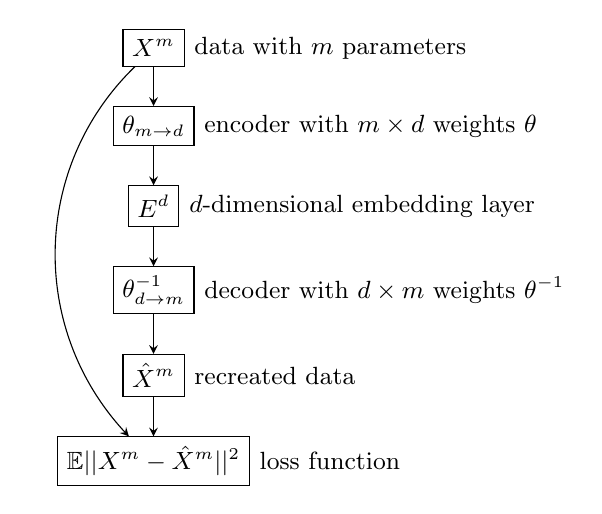
\begin{tikzpicture}[
        node distance = 5mm and 5mm,
        punkt/.style = {rectangle, draw},
        pil/.style = {black, -stealth},
        font=\small
        ]

        \node[punkt,label=right:data with $m$ parameters] (X) {$X^m$};
        \node[punkt,label=right:encoder with $m \times d$ weights $\theta$] (encoder) [below=of X] {$\theta_{m \to d}$};
        \node[punkt,label=right:$d$-dimensional embedding layer] (E) [below=of encoder] {$E^{d}$};
        \node[punkt,label=right:decoder with $d \times m$ weights $\theta^{-1}$] (decoder) [below=of E] {$\theta_{d \to m}^{-1}$};
        \node[punkt,label=right:recreated data] (Xhat) [below=of decoder] {$\hat{X}^m$};
        \node[punkt,label=right:loss function] (loss) [below=of Xhat] {$\mathbb{E}||X^{m} - \hat{X}^{m}||^2$};
          
        \draw[pil] (X) edge (encoder)
        (encoder) edge (E)
        (E) edge (decoder)
        (decoder) edge (Xhat)
        (Xhat) edge (loss)
        (X) edge[bend right=45] (loss);

      \end{tikzpicture}

\end{document}
